% Plato's Cave Allegory for SSL on EEG
% Compile standalone: pdflatex cave_allegory.tex
\documentclass[tikz,border=6pt]{standalone}
\usepackage{tikz}
\usepackage{xcolor}
\usetikzlibrary{arrows.meta, shapes, positioning, shadows}

\begin{document}
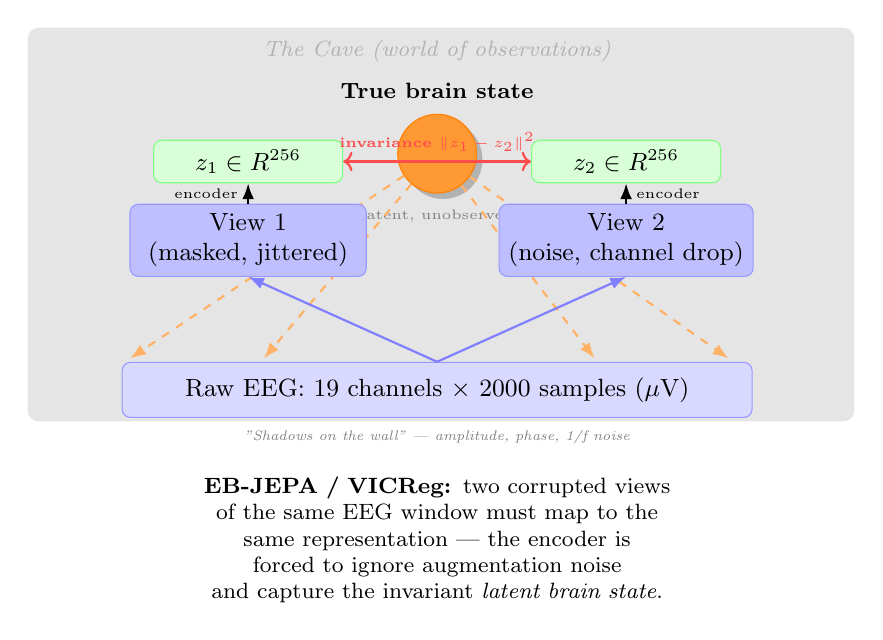
\begin{tikzpicture}[
  every node/.style={font=\small},
  arr/.style={-{Latex[length=2mm]}, thick},
  shadow/.style={fill=gray!30, draw=gray!50},
  signal/.style={fill=blue!15, draw=blue!40, rounded corners=3pt},
  latent/.style={fill=green!15, draw=green!50, rounded corners=3pt},
  wall/.style={fill=gray!60, draw=gray!80},
]

% ── cave wall (the "screen") ──────────────────────────────────────────────
\fill[gray!20, rounded corners=4pt] (-1,-1.2) rectangle (9.5, 3.8);
\node[gray!60, font=\footnotesize\itshape] at (4.2, 3.5) {The Cave (world of observations)};

% ── fire / true signal source ─────────────────────────────────────────────
\node[circle, fill=orange!80, draw=orange, minimum size=1cm, drop shadow]
  (fire) at (4.2, 2.2) {};
\node[above=2pt of fire, font=\footnotesize\bfseries] {True brain state};
\node[below=2pt of fire, font=\tiny, text=gray] {(latent, unobserved)};

% ── shadow projections (raw EEG) ─────────────────────────────────────────
\foreach \x/\lbl in {0.3/ch1, 2.0/ch2, 6.2/ch18, 7.9/ch19}{
  \draw[arr, orange!60, dashed] (fire) -- (\x, -0.4);
}
\node[signal, minimum width=8cm, minimum height=0.7cm, align=center]
  (eeg) at (4.2, -0.8) {Raw EEG: 19 channels $\times$ 2000 samples ($\mu$V)};
\node[below=1pt of eeg, font=\tiny\itshape, text=gray]
  {"Shadows on the wall" — amplitude, phase, 1/f noise};

% ── two augmented views ───────────────────────────────────────────────────
\node[signal, fill=blue!25, minimum width=3cm, align=center]
  (v1) at (1.8, 1.1) {View 1\\(masked, jittered)};
\node[signal, fill=blue!25, minimum width=3cm, align=center]
  (v2) at (6.6, 1.1) {View 2\\(noise, channel drop)};
\draw[arr, blue!50] (eeg.north) -- (v1.south);
\draw[arr, blue!50] (eeg.north) -- (v2.south);

% ── encoder ──────────────────────────────────────────────────────────────
\node[latent, minimum width=2.4cm, align=center]
  (z1) at (1.8, 2.1) {$z_1 \in \mathbb{R}^{256}$};
\node[latent, minimum width=2.4cm, align=center]
  (z2) at (6.6, 2.1) {$z_2 \in \mathbb{R}^{256}$};
\draw[arr] (v1) -- (z1) node[midway, left, font=\tiny] {encoder};
\draw[arr] (v2) -- (z2) node[midway, right, font=\tiny] {encoder};

% ── VICReg invariance pull ────────────────────────────────────────────────
\draw[arr, red!70, <->, thick] (z1.east) -- (z2.west)
  node[midway, above, font=\tiny\bfseries, text=red!70] {invariance $\|z_1-z_2\|^2$};

% ── caption ──────────────────────────────────────────────────────────────
\node[below=8pt, font=\footnotesize, align=center, text width=9cm] at (4.2,-1.5)
  {\textbf{EB-JEPA / VICReg:} two corrupted views of the same EEG window must map to the \\
   same representation — the encoder is forced to ignore augmentation noise \\
   and capture the invariant \emph{latent brain state}.};

\end{tikzpicture}
\end{document}
